% Adjust these for the path of the theme and its graphics, relative to this file
%\usepackage{beamerthemeFalmouthGamesAcademy}
\usepackage{../../beamerthemeFalmouthGamesAcademy}
\usepackage{multimedia}
\graphicspath{ {../../} }

% Default language for code listings
\lstset{language=C++,
        morekeywords={each,in,nullptr}
}

% For strikethrough effect
\usepackage[normalem]{ulem}
\usepackage{wasysym}

\usepackage{pdfpages}

% http://www.texample.net/tikz/examples/state-machine/
\usetikzlibrary{arrows,automata}

\newcommand{\modulecode}{COMP260}\newcommand{\moduletitle}{Distributed Systems}\newcommand{\sessionnumber}{5}

\begin{document}
\title{\sessionnumber: Newtonian mechanics}
\subtitle{\modulecode: \moduletitle}

\frame{\titlepage} 

\begin{frame}
	\frametitle{Learning outcomes}
	\begin{itemize}
		\item \textbf{Recall} the definitions of key concepts such as position, velocity, acceleration, force, friction and restitution
		\item \textbf{Solve} simple mathematical problems involving these key concepts
		\item \textbf{Write} programs which feature realistic physics simulations
	\end{itemize}
\end{frame}

\part{Calculus}
\frame{\partpage}

\begin{frame}{Isaac Newton (1643-1727)}
	\begin{columns}
		\begin{column}{0.2\textwidth}
			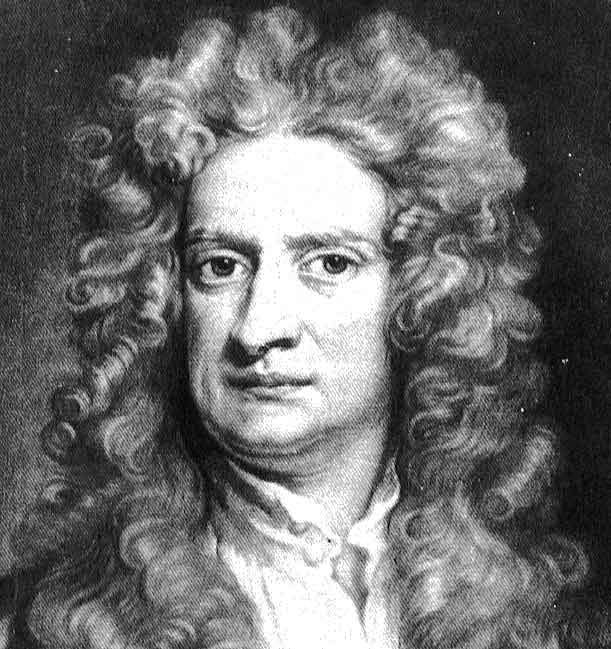
\includegraphics[width=\textwidth]{isaac_newton}
		\end{column}
		\begin{column}{0.78\textwidth}
			\begin{itemize}
				\pause\item Invented \textbf{calculus}
					\begin{itemize}
						\pause\item Study of \textbf{rates of change}
					\end{itemize}
				\pause\item Developed \textbf{laws of motion}
					\begin{itemize}
						\pause\item ``The'' laws of motion until 20th Century (Einstein's theory of relativity, quantum mechanics)
						\pause\item Still useful for motion of ``everyday'' objects (size above quantum scale, speed much lower than speed of light)
					\end{itemize}
				\pause\item Developed \textbf{laws of gravitation}
					\begin{itemize}
						\pause\item Realised that falling objects and orbiting celestial bodies are governed by the same principles
					\end{itemize}
				\pause\item Many other contributions to mathematics and physics
			\end{itemize}
		\end{column}
	\end{columns}
\end{frame}

\begin{frame}{Rates of change}
	\begin{itemize}
		\pause\item Consider a quantity that \textbf{changes over time}
		\pause\item $\text{Rate of change} = \dfrac{\text{change in quantity}}{\text{change in time}}$
	\end{itemize}
	\pause
	\begin{columns}
		\begin{column}{0.4\textwidth}
			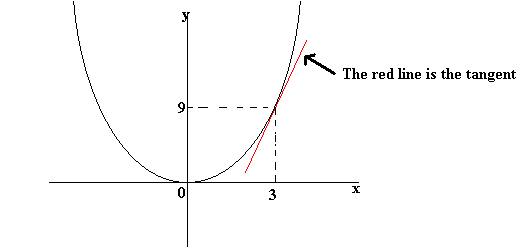
\includegraphics[width=\textwidth]{gradient}
		\end{column}
		\begin{column}{0.58\textwidth}
			Same as the \textbf{gradient} of a graph (from GCSE maths):
			$$\text{gradient} = \dfrac{\text{change in } y}{\text{change in } x}$$
		\end{column}
	\end{columns}
	\begin{itemize}
		\pause\item The \textbf{derivative} of a quantity $x$ with respect to time $t$ is \textbf{the rate of change}
			of $x$ with respect to $t$
		\pause\item Denoted $\dfrac{dx}{dt}$
		\pause\item The mathematical process of finding $\dfrac{dx}{dt}$ given $x$ is called \textbf{differentiation}
	\end{itemize}
\end{frame}

\begin{frame}{Derivatives -- example}
	\begin{itemize}
		\pause\item A car is driving along a straight road at a constant speed
		\pause\item In half an hour, it covers a distance of 20 miles
		\pause\item Its average speed is $\dfrac{20 \text{ miles}}{0.5 \text{ hours}} = 40 \text{ miles per hour}$
		\pause\item In other words...
			\begin{itemize}
				\pause\item \textbf{Distance travelled} is a quantity varying with time
				\pause\item We call the rate of change of this quantity \textbf{speed}
				\pause\item If $x$ is distance travelled and $t$ is time, then we have
					$$\dfrac{dx}{dt} = \dfrac{20}{0.5} = 40$$
			\end{itemize}
	\end{itemize}
\end{frame}

\begin{frame}{Integration}
	\begin{itemize}
		\pause\item Given $\dfrac{dx}{dt}$, find $x$
		\pause\item $x$ is the \textbf{integral} of $\dfrac{dx}{dt}$
		\pause\item The process of finding $x$ is called \textbf{integration}, the opposite of differentiation
		\pause\item We are interested in \textbf{numerical integration}
			\begin{itemize}
				\pause\item I.e.\ integration by computer calculation, not by mathematician with pen and paper...
			\end{itemize}
	\end{itemize}
\end{frame}

\begin{frame}{Euler method}
	\begin{itemize}
		\pause\item If we know values of $x$ and $\frac{dx}{dt}$ at time $t$, we can \textbf{estimate}
			the value of $x$ at time $t+h$
		\pause\item Formula:
			$$ x(t+h) \approx x(t) + h \times \frac{dx}{dt}(t) $$
		\pause\item $\frac{dx}{dt}$ is rate of change, i.e.\ how much $x$ changes by if $t$ changes by $1$
		\pause\item So $h \times \frac{dx}{dt}$ is how much $x$ changes by if $t$ changes by $h$
	\end{itemize}
\end{frame}

\begin{frame}{Euler method}
	\begin{center}
		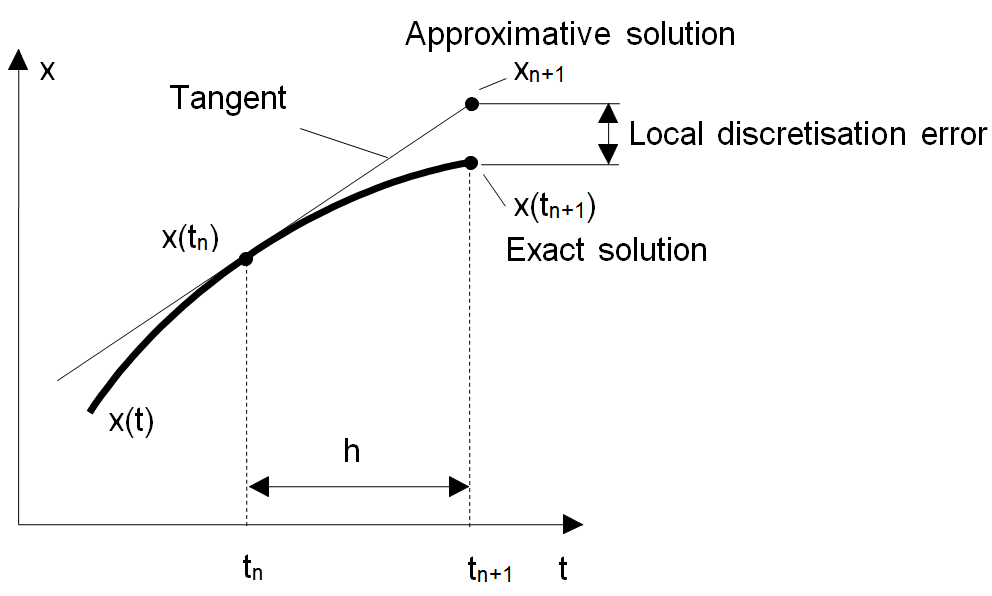
\includegraphics[width=0.6\textwidth]{euler_method}
	\end{center}
	\begin{itemize}
		\pause\item If $\frac{dx}{dt}$ does not change between $t$ and $t+h$, this gives the \textbf{exact} answer;
			otherwise there will be an \textbf{error}
		\pause\item If $h$ is small enough, the error should also be small...
		\pause\item There are more advanced forms of numerical integration which give smaller errors
	\end{itemize}
\end{frame}

\begin{frame}{Calculus with vectors}
	\begin{itemize}
		\pause\item Can talk about rate of change of vectors as well
		\pause\item If $x$ is an $n$-vector, then so is $\frac{dx}{dt}$
		\pause\item Each component of $\frac{dx}{dt}$ is the rate of change of the corresponding component of $x$
	\end{itemize}
\end{frame}


\part{Newtonian Mechanics}
\frame{\partpage}

\begin{frame}{Calculus: differentiation}
	\begin{columns}
		\begin{column}{0.58\textwidth}
			\begin{itemize}
				\pause\item The \textbf{derivative} $\dfrac{dx}{dt}$ of a quantity $x$ with respect to time $t$ is \textbf{the rate of change} of $x$ with respect to $t$
				\pause\item i.e. how much $x$ changes by if $t$ changes by $1$
			\end{itemize}
		\end{column}
		\begin{column}{0.4\textwidth}
			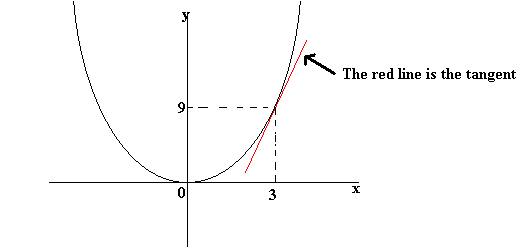
\includegraphics[width=\textwidth]{gradient}
		\end{column}
	\end{columns}
	\begin{itemize}
		\pause\item Equivalent to the \textbf{gradient} of a graph, $\dfrac{\text{change in } y}{\text{change in } x}$		
		\pause\item For moving objects:
		\begin{itemize}
			\pause\item \textbf{Velocity} is the derivative of \textbf{displacement}
			\pause\item \textbf{Acceleration} is the derivative of \textbf{velocity}
			\pause\item NB \textbf{speed} is the \textbf{magnitude} of velocity
		\end{itemize}
	\end{itemize}
\end{frame}

\begin{frame}{Calculus: integration}
	\begin{itemize}
		\pause\item The opposite of differentiation: $x$ is the \textbf{integral} of $\dfrac{dx}{dt}$
		\pause\item We are interested in \textbf{numerical integration}, i.e. by computer calculation
		\pause\item \textbf{Euler method}: given $x$ and $\frac{dx}{dt}$ at time $t$, we can \textbf{estimate} the value of $x$ at time $t+h$:
	\end{itemize}
	\begin{columns}
		\begin{column}{0.58\textwidth}
			\pause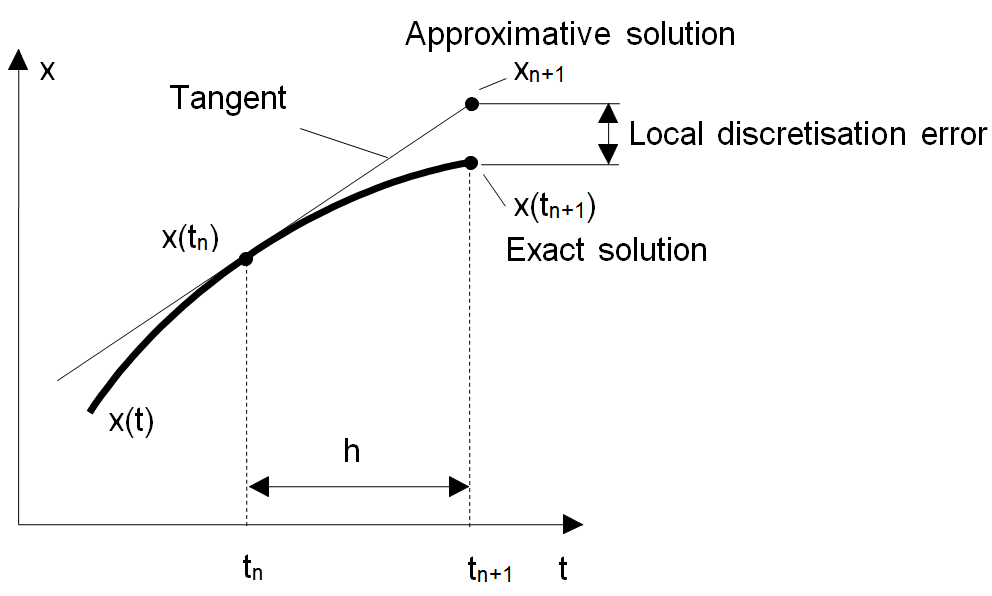
\includegraphics[width=\textwidth]{euler_method}
		\end{column}
		\begin{column}{0.4\textwidth}
			\pause $$ x(t+h) \approx x(t) + h \times \frac{dx}{dt}(t) $$
		\end{column}
	\end{columns}
\end{frame}

\begin{frame}{Basic simulation loop}
	\begin{itemize}
		\pause\item For each object, store its position $\boldsymbol{x}$ and velocity $\boldsymbol{v}$
		\pause\item On each time step $\Delta{t}$:
		\begin{itemize}
			\pause\item Find the new position using numerical integration, $\boldsymbol{x}' = \boldsymbol{x} + $$\boldsymbol{v}\Delta{t}$
			\pause\item Calculate the forces acting on the object, and thus the acceleration $\boldsymbol{a}$ from Newton's second law, $\boldsymbol{F} = m\boldsymbol{a}$
			\pause\item Find the new velocity using numerical integration, $\boldsymbol{v}' = \boldsymbol{v} + $$\boldsymbol{a}\Delta{t}$
		\end{itemize}
	\end{itemize}
\end{frame}

\begin{frame}{Newton's Laws of Motion}
	\begin{center}
		\pause An object remains at rest or moves at constant velocity unless acted upon by an external force
		
		\vspace{2ex}
		
		\pause $\boldsymbol{F} = m\boldsymbol{a}$: The sum of forces acting upon an object is equal to its mass multiplied by its acceleration
		
		\vspace{2ex}
		
		\pause When one body exerts a force on another, the second body exerts an equal and opposite force on the first
	\end{center}
\end{frame}

\begin{frame}{Basic collision response}
	\begin{columns}
		\begin{column}{0.4\textwidth}
			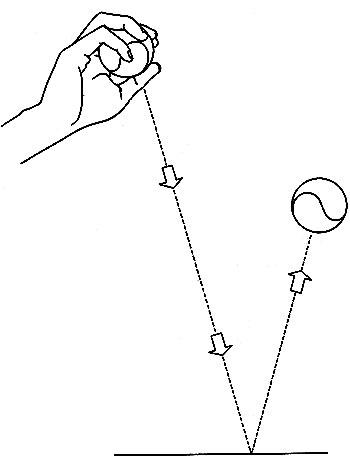
\includegraphics[width=\textwidth]{bounce_reflection}
		\end{column}
		\begin{column}{0.58\textwidth}
			\begin{itemize}
				\pause\item For an \textbf{elastic collision}, the component of velocity parallel to the \textbf{surface normal}
					is \textbf{reversed}
				\pause\item E.g.\ if the surface is the $xz$ plane, flip the $y$ component
				\pause\item For an \textbf{inelastic collision}, some velocity is lost
				\pause\item Flip the $y$ component and multiply it by something between $0$ and $1$
			\end{itemize}
		\end{column}
	\end{columns}
\end{frame}



\part{Sprint review}
\frame{\partpage}

\end{document}
